\documentclass[a4paper]{article}
\usepackage[utf8]{inputenc}
\usepackage{t1enc}
\usepackage[magyar]{babel}
\usepackage[pdftex]{graphicx}
\usepackage{graphics}
\usepackage{epstopdf}
\usepackage{sidecap}
\usepackage{caption}
\usepackage{subcaption}
\usepackage{pifont}
\usepackage{shadow}

\begin{document}
\includegraphics[scale=0.2]{totoro.png}

\begin{figure}[bp]
\center
\resizebox{80mm}{!}{
\rotatebox{-90}{
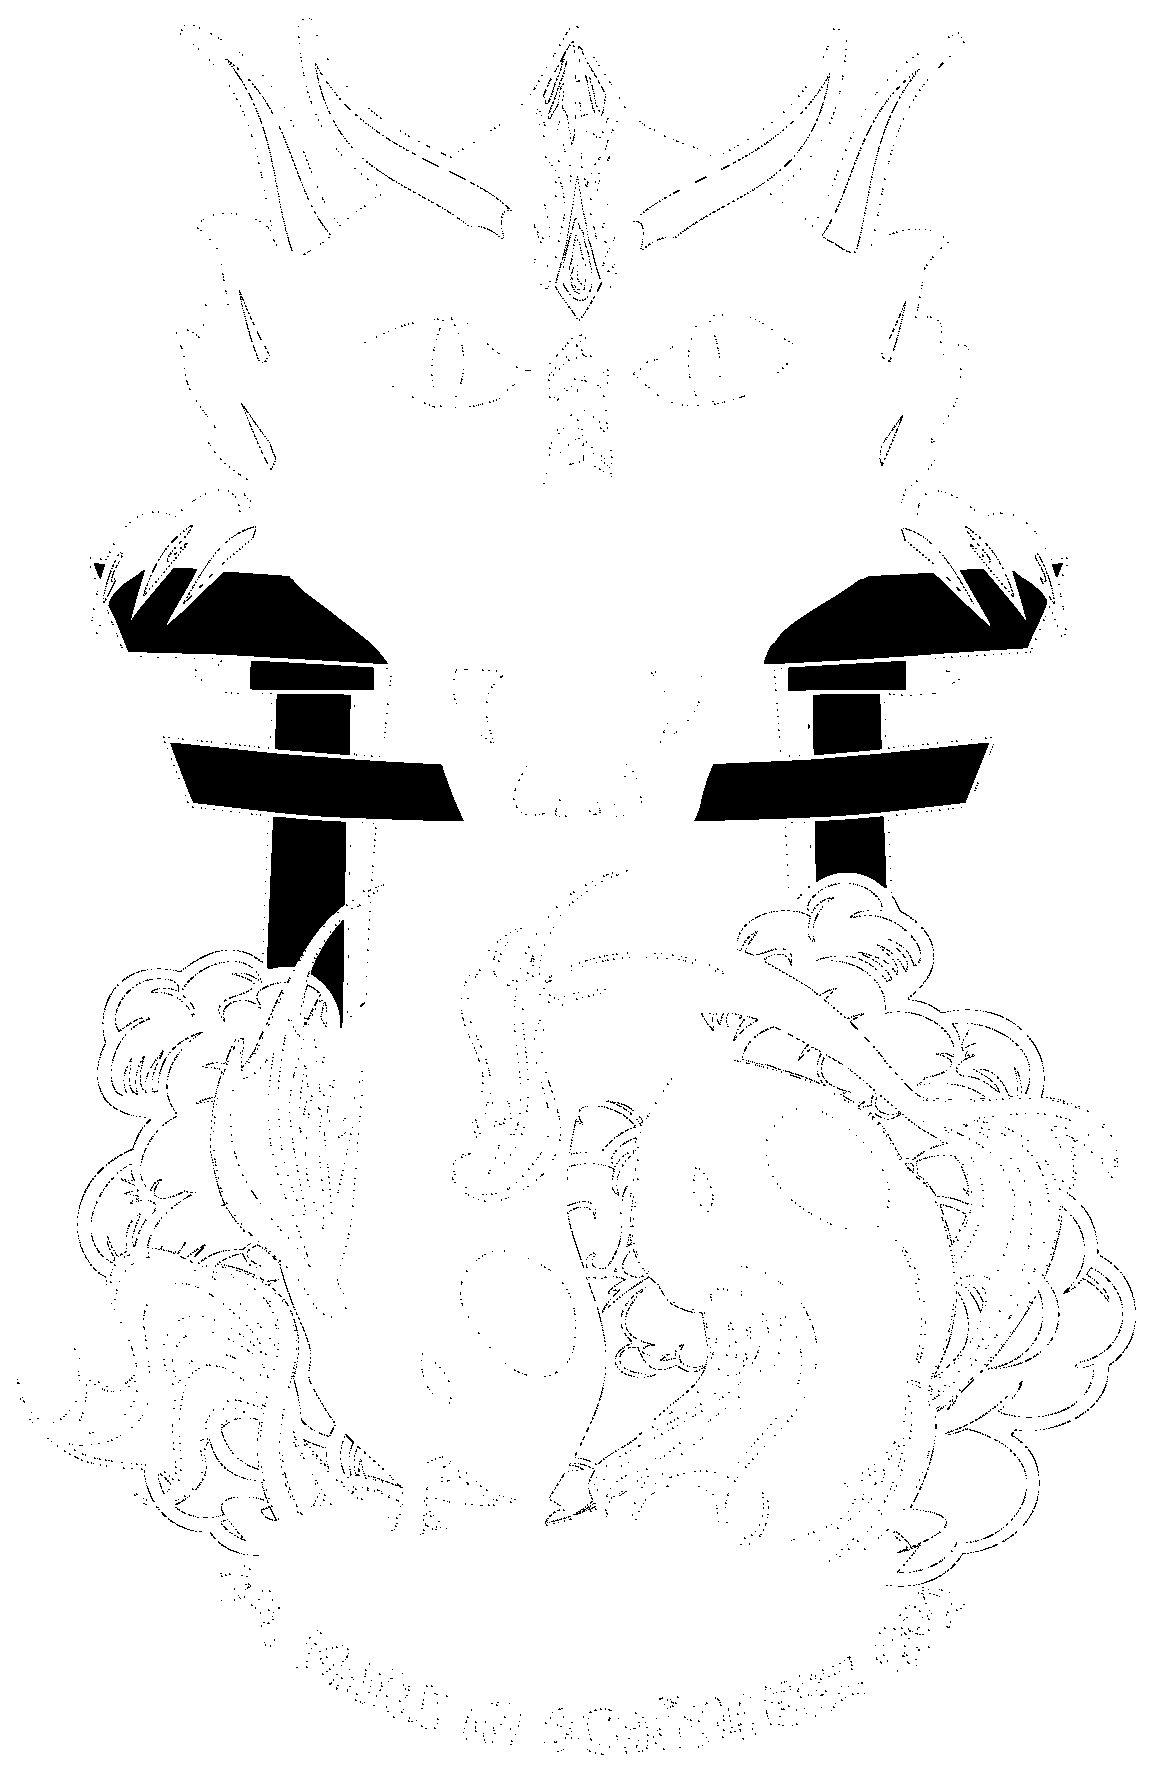
\includegraphics[scale=0.2]{sarkany.eps}}}
\caption{A \LaTeX\ órák mestere}
\label{fig:sarkany}
\end{figure}
\begin{figure}[h!]
\centering
\reflectbox{%
\includegraphics[width=0.5\textwidth]{totoro.png}}
\caption{A kep cimet itt adjuk meg}
\end{figure}
\begin{SCfigure}
\centering
\includegraphics[width=0.55\textwidth]{totoro.png}
\caption{Az afrikai elefánt (Loxodonta africana) a Földön ma élő legerősebb és
legnagyobb szárazföldi emlősállat. Eredendően szavannákon él, ám
kitűnően alkalmazkodik ahhoz, hogy Afrika más, különböző éghajlatú
területein is megélhessen, azonban élőhelyének közelében mindenképpen
ivóvízforrás kell hogy legyen.}
\end{SCfigure}

\begin{figure*}
\centering
\begin{subfigure}[t]{0.3\textwidth}
\centering
\includegraphics[width=\textwidth]{elefant.jpg}
\caption{Afrikai elefánt}
\end{subfigure}\\
\begin{subfigure}[t]{0.3\textwidth}
\centering
\includegraphics[width=\textwidth]{totoro.png}
\caption{Totoroi elefánt}
\end{subfigure}\\
\begin{subfigure}[t]{0.3\textwidth}
\centering
\includegraphics[width=\textwidth]{dumbo.jpg}
\caption{Walt-Disney elefánt}
\end{subfigure}
\caption{A világ elefántjai}
\end{figure*}

\mbox{sima doboz keret nélkül}
\fbox{sima keretezett doboz}
{\setlength{\fboxrule}{3pt} \fbox{vastag keretes doboz}}
{\setlength{\fboxsep}{0pt} \fbox{térközmentes keretes doboz}}

Ez \raisebox{2ex}{egy} sor.

{\setlength{\sboxrule}{3pt} \shabox{vastag keretes
doboz}}
{\setlength{\sboxsep}{0pt} \shabox{térközmentes
keretes doboz}}
{\setlength{\sdim }{10pt} \shabox{Nagy árnyékos
doboz}}

\dots
\fbox{\parbox[t][50mm]{90mm}{\vfill \raggedleft
\hrulefill \shabox{\scriptsize Kovács Alajos} \
\
\tiny nyugdíjas főtörzsőrmester \\[6pt]
\ding{38} +36-1-234-5678 \\
\ding{41} alajos@kovacs.hu \vfill}}
\fbox{\rule{0pt}{1cm}ez a doboz legalább 1\,cm magas}
\fbox{ez} \fbox{egy} \fbox{egyenetlen} \fbox{dobozsor}
\fbox{\strut ez} \fbox{\strut már} \fbox{\strut egyenletes}
\fbox{\strut dobozsor} ... $(\sqrt{g} + \sqrt{h})$ csúnya, de
$\left(\sqrt{\mathstrut g} + \sqrt{\mathstrut h}\right)$
szép.

\end{document}